\documentclass[pdftex,
               12pt,
               DIV=12,
               a4paper,
               twoside,
               parskip=half,
               abstract=true,
               dvipsnames]{scrartcl}

\usepackage[american,naustrian]{babel}
\usepackage[utf8]{inputenc}
\usepackage[T1]{fontenc}
\usepackage{lineno}
\linenumbers

% weitere Packages, welche Sie verwenden moechten
%Mathe Werkzeuge
\usepackage{amsmath}
\usepackage{amsfonts}
\usepackage{bchart}
\usepackage{nicefrac}
\usepackage{array}

%fuer Bilder
\usepackage{graphicx}
\usepackage{caption}
\usepackage{subcaption}

%Farben und Grafiken
\usepackage{tikz}

%Pfad zu den Bildern
\graphicspath{ {images/} }

%fuer Referenzen
\usepackage{hyperref}
\usepackage[ngerman]{cleveref}

%fuer Bibliographie
\usepackage[numbers]{natbib}

%eigene Befehle
\newcommand{\N}{\ensuremath{\mathbb{N}}}

% Info zu Autoren und Titel
\author{Andreas Auer, Philipp Fuchs,\\ Sarah G\"otz, Moritz Kondmann}
\title{Schwarmintelligenz}

\begin{document}
\maketitle

\begin{abstract}
Diese Arbeit beschäftigt sich mit den grundlegenden Prinzipien der Schwarmintelligenz und stellt zwei darauf basierende Algorithmen vor. Im Fokus stehen der Ameisenalgorithmus (Ant Colony Optimization, ACO) und die Partikelschwarmoptimierung (Particle Swarm Optimization, PSO), die sich durch selbstorganisierte und dezentrale Entscheidungsmechanismen auszeichnen. Neben einer detaillierten Erläuterung ihrer Funktionsweise werden ihre jeweiligen Stärken und Schwächen analysiert. Zudem wird aufgezeigt, in welchen Anwendungsbereichen diese Algorithmen zum Einsatz kommen, beispielsweise in der Optimierung von Routen und in kontinuierlichen Optimierungsprozessen.
\end{abstract}


\section{Schwarmintelligenz Allgemein}
Schwarmintelligenz beschreibt das kollektive Verhalten von dezentralisierten, selbstorganisierten Systemen. Ein solches Kollektiv zeichnet sich durch die dezentrale F\"uhrung der Gruppe, die Selbstorganisation eines jeden Individuums und durch das Zusammenspiel der einzelnen Schwarmmitglieder untereinander aus. In der Natur zeigen Tiere diese Verhaltensweisen, um wichtige Aufgaben wie die Nahrungssuche, die Suche nach einem Rastplatz oder den Schutz vor Feinden zu bew\"altigen. Beispiele sind zum einen Ameisenkolonien und zum anderen Vogel- oder Fischschw\"arme. \cite[vgl.][]{KennedyEberhart01}

In der Informatik wird das Prinzip der Schwarmintelligenz zur Entwicklung von leistungsf\"ahigen Optimierungsalgorithmen, wie dem Ameisenalgorithmus oder der Partikelschwarmoptimierung genutzt. Diese Verfahren nutzen das koordinierte Verhalten vieler einfacher Einheiten, die durch lokale Interaktionen komplexe Probleme effizient lösen können. Sie überzeugen durch ihre Flexibilität, Widerstandsfähigkeit und Skalierbarkeit, wodurch sie für zahlreiche Optimierungsaufgaben besonders geeignet sind. \cite[vgl.][]{KennedyEberhart01, DorigoStuetzle04}


\section{Ameisenalgorithmus ACO}
\subsection{Einleitung}
Eines der wesentlichen Probleme der Informatik ist die Optimierung komplexer Routen. Daf\"ur gibt es verschiedene L\"osungsans\"atze. Ein recht erfolgreicher hat seinen Ursprung in der Natur: Ameisen bilden einen Schwarm und finden so gemeinsam durch eigens entwickelte, simple, aber clevere Mechanismen k\"urzeste Wege zu Nahrungsquellen oder \"Ahnlichem. Dieses Verhalten bildet die Grundlage f\"ur die sogenannte Ant Colony Optimization (ACO), eine von Ameisenkolonien inspirierte Metaheuristik, die zur bestm\"oglichen L\"osung komplexer, kombinatorischer Optimierungsprobleme eingesetzt wird. Diese Methode wurde in den 1990er Jahren von Marco Dorigo und seinen Kollegen entwickelt und wird seither weiterentwickelt und f\"ur verschiedenste Probleme verwendet und adaptiert. \cite[vgl.][]{DorigoStuetzle04}


\subsection{Biologie}
\begin{figure}[h]
	\centering
	\begin{subfigure}{0.45\textwidth}
		\includegraphics[width=\linewidth, page=2]{aco_biology}
		\caption{} \label{subfig:ACO_biologie_a}
	\end{subfigure}
	\begin{subfigure}{0.45\textwidth}
		\includegraphics[width=\linewidth, page=3]{aco_biology}
		\caption{} \label{subfig:ACO_biologie_b}
	\end{subfigure}
	\begin{subfigure}{0.45\textwidth}
		\includegraphics[width=\linewidth, page=4]{aco_biology}
		\caption{} \label{subfig:ACO_biologie_c}
	\end{subfigure}
	\caption{Entwicklung der Pheromonverteilung in der Natur \cite[vgl.][]{Engelbrecht07}}
\end{figure}

Die Strategie, nach der Ameisen in der Natur vorgehen und auf welcher auch das Prinzip der ACO-Algorithmen basiert, sind Pheromone. Ameisen produzieren diese Pheromone und hinterlassen sie auf ihren Routen, wodurch eine einfache Kommunikation und Orientierung der Kolonie m\"oglich ist.
Folgendermaßen gehen die Ameisen vor: Zu Beginn bewegt sich eine Ameise zuf\"allig in eine beliebige Richtung. W\"ahrenddessen hinterl\"asst sie Pheromone, die von den folgenden Ameisen wahrgenommen werden [\cref{subfig:ACO_biologie_a}]. Mit zunehmender Anzahl an Ameisen wird mehr Pheromon auf allen Pfaden verteilt - insbesondere steigt die Pheromonkonzentration auf den k\"urzesten Pfaden, da diese schneller zur\"uckgelegt und somit h\"aufiger markiert werden. Zudem sind Wege mit h\"oherer Pheromonkonzentration attraktiver f\"ur nachfolgende Ameisen, wodurch diese Wege mit gr\"o\ss erer Wahrscheinlichkeit gegangen werden. W\"ahrenddessen verschwindet Pheromon auf weniger genutzten Routen durch Verdunstung allm\"ahlich [\cref{subfig:ACO_biologie_b}]. Nach gewisser Zeit entsteht so eine recht deutliche Pheromonverteilung. Die wenigen Ausreißer dienen der Erkundung - f\"ur den Fall, dass beispielsweise ein neuer, k\"urzerer Pfad entdeckt wird. Durch diese Mechanismen ist es den Ameisen m\"oglich, sich auf die effizienten Wege zu fokussieren, w\"ahrend gleichzeitig die M\"oglichkeit der Erkundung neuer Alternativen erhalten bleibt [\cref{subfig:ACO_biologie_c}].  Dieses Verhalten l\"asst sich auf ACO-Algorithmen \"ubertragen, wobei Populationen k\"unstlicher Ameisen verwendet werden, die in einer graphischen Darstellung des Problems navigieren. \cite[vgl.][]{DorigoStuetzle04}


\subsection{Problem des Handelsreisenden}
Das Problem des Handelsreisenden (Travelling Salesman Problem, TSP) ist ein fundamentales kombinatorisches Optimierungsproblem in der Graphentheorie. Es beschreibt das Problem eines Verk"aufers, der ausgehend von seiner Heimatstadt, die k"urzeste Tour finden will um alle St"adte seiner Kunden genau einmal zu besuchen und anschließend zur\"uckzukehren. Mathematisch kann das Problem als vollst\"andig gewichteter Graph beschrieben werden, wobei die optimale L\"osung, einem Hamiltonschen Kreis mit minimaler Kantensumme entspricht. [\cref{fig:ACO_tspgraph}]. Die Knoten repr\"asentieren dabei die St\"adte der Kunden und die Kantengewichte die Distanz zwischen zwei St\"adten. \cite[vgl.][]{DorigoStuetzle04}

	\begin{figure}[h]
		\centering
		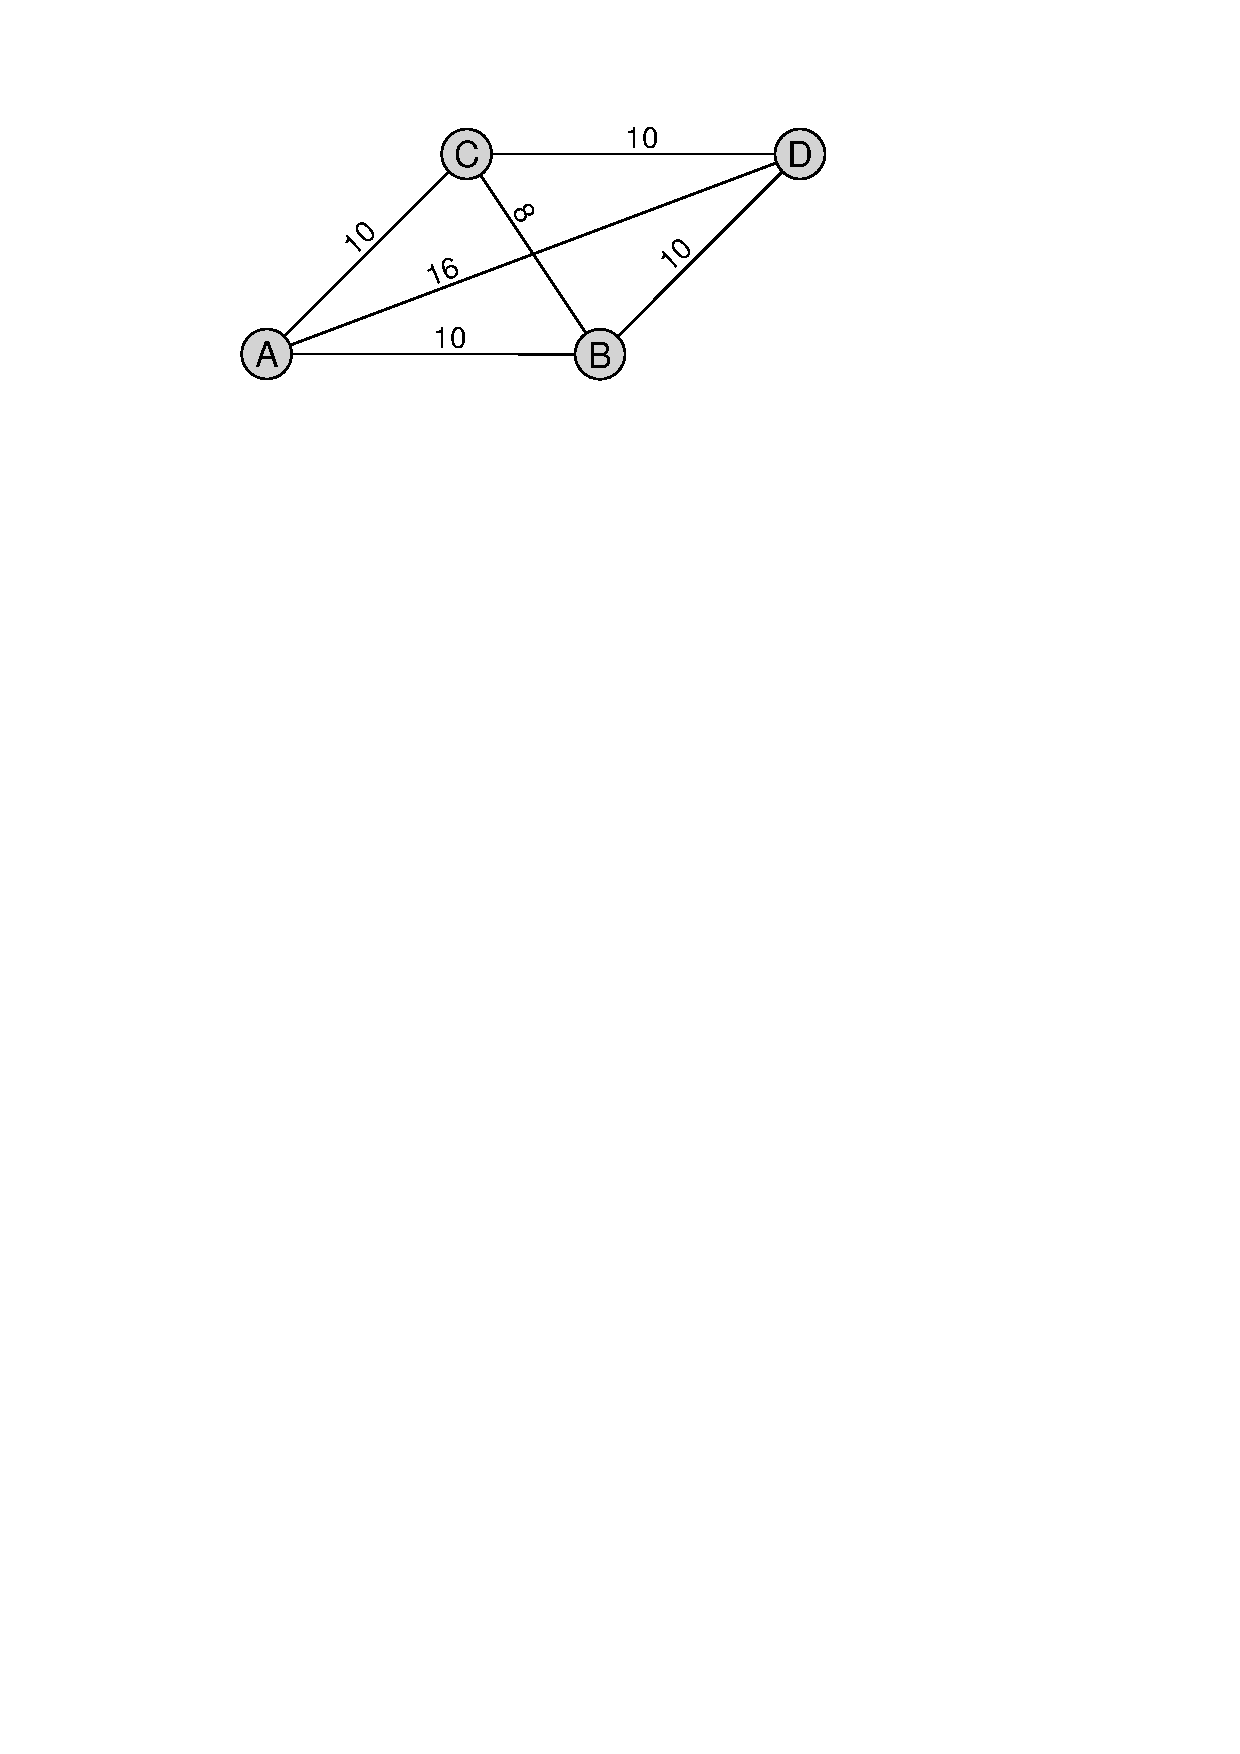
\includegraphics[width=0.5\textwidth, page=1]{aco_tspgraph}
		\caption{TSP Beispielgraph} \label{fig:ACO_tspgraph}
	\end{figure}


\subsubsection{L\"osungsansatz: Brute Force}
Der Brute Force Ansatz l\"ost das Problem, indem er die Kantensummen aller m\"oglichen Permutationen berechnet, und anschlie\ss end die Tour mit der minimalen Gesamtdistanz ausw\"ahlt. Die Anzahl der Permutationen entspricht dabei $\frac{(n-1)!}{2}$, wobei n die Anzahl der Knoten im Graph ist. \cite[vgl.][]{Rimscha17}

\begin{table}[ht]
	\begin{center}
	\begin{tabular}{|c|l|} \hline
		\textbf{Anzahl St\"adte} & \textbf{Anzahl Touren} \\
		\hline
		4 & 3 \\
		5 & 12 \\
		10 & 181 440 \\
		15 & 43 589 145 600 \\
		20 & 60 822 550 204 416 000\\
		\hline
	\end{tabular}
	\caption{Brute Force Komplexit\"at} \label{tab:ACO_bruteforce}
		\end{center}
\end{table}

Ein wesentlicher Vorteil dieser Methode ist, dass durch Berechnen aller m\"oglichen Permutationen garantiert eine optimale L\"osung gefunden wird. Jedoch nimmt die Anzahl der Permutationen f\"ur gro\ss e nat\"urliche Zahlen $n$ extrem schnell zu, sodass dieser Ansatz nur f\"ur kleine Eingabegr\"o\ss en effizient berechenbar ist [\cref{tab:ACO_bruteforce}].


\subsubsection{L\"osungsansatz: Greedy Algorithmus - Nearest Neighbor}
Eine Alternative stellt das Verwenden eines Greedy Algorithmus (z.B. Nearest Neighbor) dar. Dieser trifft mit jedem Schritt eine lokal optimale Entscheidung und w\"ahlt somit immer die Stadt mit der geringsten Entfernung um eine Tour zu konstruieren. \cite[vgl.][]{DorigoStuetzle04}

Am Beispielgraphen [\cref{fig:ACO_greedygraph}] startet der Algorithmus eine Tour bei Knoten $A$ und kann zun\"achst zwischen den Knoten $B$, $C$ und $D$ w\"ahlen. Aufgrund der geringeren Distanz zu Knoten $B$ und $C$ wird der Algorithmus einen der beiden Knoten ausw\"ahlen. F\"allt die Entscheidung auf $B$, so wird anschlie\ss end $C$ bevorzugt, da die Kante $\overline{BC}$ die geringeren Kosten aufweist. Nun bleibt als letzte Wahl nur noch der Knoten $D$ \"ubrig, von dem aus es mit $\overline{DA}$ zur\"uck zum Startknoten $A$ geht.

Ein wesentlicher Nachteil dieses Ansatzes besteht darin, dass eine lokal optimale Entscheidung nicht zwangsl\"aufig zu einem globalen Optimum f\"uhrt. Es kann z.B. vorkommen dass der Algorithmus am Schluss gezwungen ist, eine deutlich teurere Kante zum Startknoten zu w\"ahlen. Wie in \cref{fig:ACO_greedygraph} zu sehen f\"uhrt dies zu einer Gesamtl\"ange der Tour von 44, w\"ahrend eine optimale Tour (z.B. $A \rightarrow B \rightarrow D \rightarrow C \rightarrow A$) nur eine L\"ange von 40 aufweist. \cite[vgl.][]{DorigoStuetzle04}

\begin{figure}[h]
	\begin{center}
		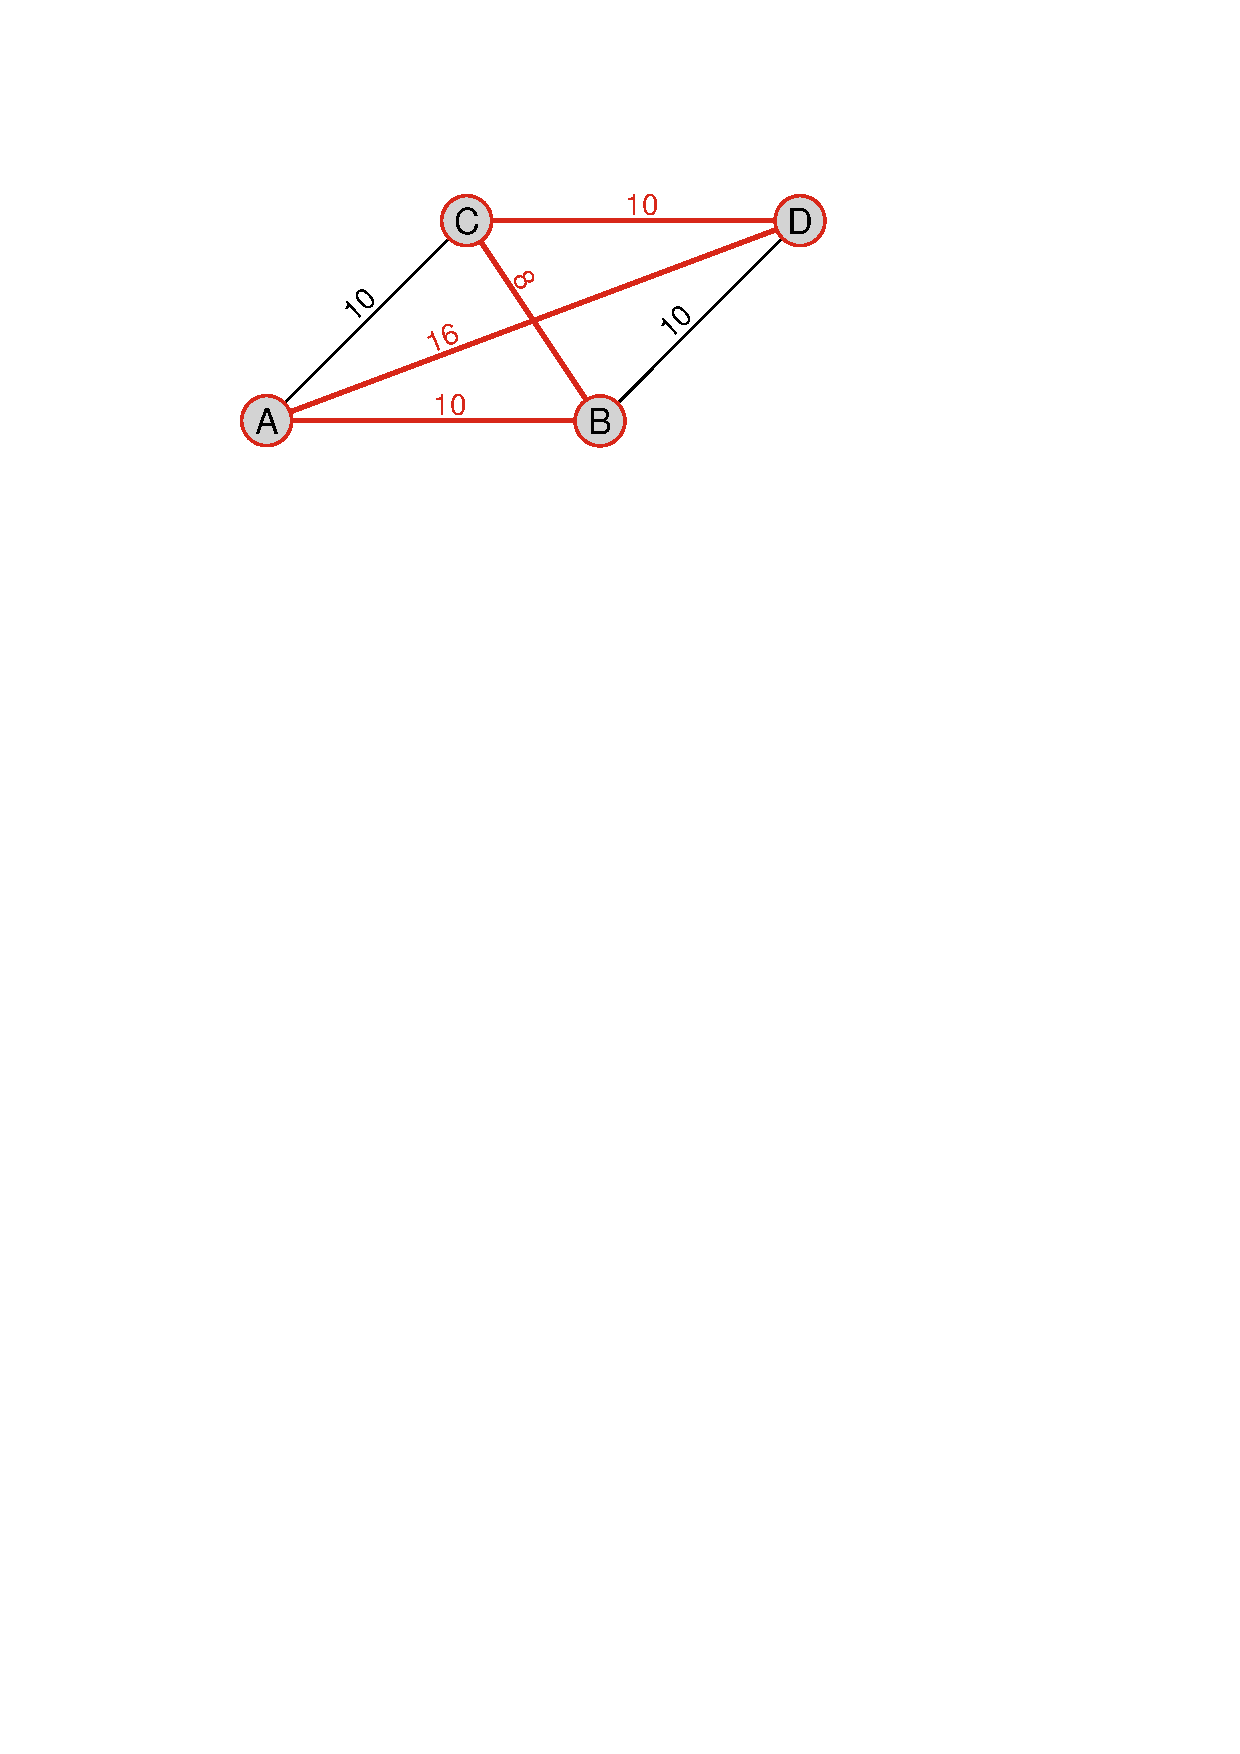
\includegraphics[width=0.5\linewidth, page=1]{aco_nearest_neighbor}
	\end{center}
	\caption{Greedy Algorithmus L\"osung} \label{fig:ACO_greedygraph}
\end{figure}


\subsubsection{L\"osungsansatz: ACO Algorithmus}
Der ACO l\"ost das TSP-Problem unter Verwendung von k\"unstlichen Ameisen, bei denen die Entscheidungsfindung echter Ameisen mittels einer Wahrscheinlichkeitsfunktion simuliert wird. Dabei werden neben den heuristischen Informationen wie z.B. der Distanz zwischen zwei St\"adten auch historische Informationen (Pheromone) ber\"ucksichtigt. Diese dienen als Ged\"achtnis f\"ur vergangene gute L\"osungen, da Kanten die zuvor Teil einer guten L\"osung waren, eine h\"ohere Pheromonkonzentration aufweisen. \cite[vgl.][]{DorigoStuetzle04}

\textbf{Ablauf des ACO Algorithmus:}

\begin{enumerate}
	\item Pheromonwerte aller Kanten initialisieren.
	\item Ameisen zuf\"allig auf die Knoten des Graphen verteilen. \label{enum:ACO_algo_2}
	\item Jede Ameise konstruiert eine eigene, wahrscheinlichkeitsbasierte L\"osung und ermittelt deren Qualit\"at
	\item Pheromonwerte aktualisieren \label{enum:ACO_algo_4}
\end{enumerate}

Die \crefrange{enum:ACO_algo_2}{enum:ACO_algo_4} werden so lange wiederholt, bis die L\"osung konvergiert oder ein Abbruchkriterium erreicht ist. \cite[vgl.][]{DorigoStuetzle04}


\subsection{Anwendung des Algorithmus}
Angewandt an dem TSP-Beispiel l\"asst sich der Ablauf des Algorithmus nun veranschaulichen. In dieser Veranschaulichung wird der Algorithmus f\"ur eine einzelne k\"unstliche Ameise durchlaufen. In der realen Anwendung des Algorithmus werden meist mehrere Ameisen zugleich losgeschickt.

Im ersten Schritt werden die Pheromone initialisiert - eine geringe Menge an Pheromon wird gleichm\"a\ss ig auf alle Kanten des zuvor definierten Graphen [\cref{fig:ACO_tspgraph}] verteilt.
Beim Start der Ameise in Punkt $A$ steht diese nun vor der Wahl zwischen den Kanten $\overline{AB}$, $\overline{AC}$ und $\overline{AD}$. Die Entscheidung \"uber den n\"achstgew\"ahlten Knoten basiert auf einer Wahrscheinlichkeitsregel. Die Wahrscheinlichkeit $P_{ij}$ einer sich aktuell in Knoten $i$ befindenden Ameise, den Knoten $j$ zu w\"ahlen ist gegeben durch \[P_{ij}=\frac{\tau_{ij}^\alpha \cdot \eta_{ij}^\beta}{\sum_{k \in N_i}\tau_{ik}^\alpha \cdot \eta_{ik}^\beta}\,.\]
Dabei werden folgende Parameter herangezogen:
\begin{itemize}
	\item $\tau_{ij}$ repr\"asentiert die Pheromonkonzentration auf der Kante $\overline{ij}$; diese wird nach Durchlauf aller zugleich gestarteten Ameisen jeweils aktualisiert.
	\item $\eta_{ij}$ ist der heuristische Wert und entspricht typischerweise dem Kehrwert der Distanz ($\nicefrac{1}{d_{ij}}$) oder Zeit, wodurch k\"urzere Wege bevorzugt werden (auch Ma\ss\ der Attraktivit\"at oder Sichtbarkeit genannt); diese Information ist bereits vor Beginn des Algorithmus bekannt.
	\item $\alpha, \beta$ sind Gewichtungsfaktoren, die den relativen Einfluss von Pheromoninformation und heuristischem Wert steuern.
	\item $N_i$ stellt die Menge der noch nicht von der Ameise besuchten Nachbarknoten von $i$ dar; f\"ur - unter anderem - diese Information verf\"ugen die k\"unstlichen Ameisen \"uber ein Ged\"achtnis.
\end{itemize}

Diese Formel zur Berechnung der Wahrscheinlichkeit wird h\"aufig, je nach Problemstellung und ben\"otigter Algorithmus-Variante leicht abge\"andert, Parameter \"andern sich oder werden hinzugef\"ugt. Die hier beschriebene und genutzte Formel ist eine Basisversion, von welcher viele Varianten abgeleitet werden - sie stammt aus dem urspr\"unglichen ACO-Algorithmus von M. Dorigo. \cite[vgl.][]{DorigoStuetzle04}

Unter Verwendung dieser Wahrscheinlichkeitsformel und dem initialisierten Pheromon lassen sich die Wahrscheinlichkeiten der Kanten des Graphen berechnen. Anschlie\ss end wird ein Zufallswert zwischen 0 und 1 bestimmt, nachdem die zu gehende Kante gew\"ahlt wurde. Bei den Wahrscheinlichkeiten
\begin{center}
	\begin{tabular}{ c c c }
		$P_{AB}$ &=& 0.38 \\
		$P_{AC}$ &=& 0.38 \\
		$P_{AD}$ &=& 0.24
	\end{tabular}
\end{center}
und einem Zufallswert 0.30, welcher auf $P_{AB}$ abbildet, wird die Kante $\overline{AB}$ gew\"ahlt [\cref{subfig:ACO_wahrscheinlichkeiten_a}]. Nach diesem Vorgehen bewegt sich die k\"unstliche Ameise nun durch den Graphen. In Stadt B hat sie die Wahl zwischen Kante $\overline{BC}$ und $\overline{BD}$ (zu $A$ kann sie schlie\ss lich noch nicht zur\"uck, da alle Knoten besucht werden m\"ussen). Nach Berechnung von Wahrscheinlichkeiten
\begin{center}
	\begin{tabular}{ c c c }
		$P_{BC}$ &=& 0.56 \\
		$P_{BD}$ &=& 0.44
	\end{tabular}
\end{center}
und einem Zufallswert 0.73, welcher auf $P_{BD}$ abbildet, geht die Ameise nach Knoten $D$ [\cref{subfig:ACO_wahrscheinlichkeiten_b}]. Hier kommt der Vorteil der Zufallskomponente zum Tragen, da so, trotz h\"oherer Wahrscheinlichkeit der Kante $\overline{BC}$, die Kante $\overline{BD}$ entdeckt und auch gegangen wird. Die Wahrscheinlichkeit, den letzten noch nicht verwendeten Knoten $C$ zu besuchen, liegt trivialerweise bei eins und damit wird Kante $\overline{CD}$ gegangen. Schlussendlich beibt noch die Kante $\overline{AC}$ zur\"uck zum Start und damit ist die Tour vollendet, welche in dem Fall tats\"achlich dem k\"urzesten Weg entspricht [\cref{subfig:ACO_wahrscheinlichkeiten_c}]. \cite[vgl.][]{DorigoStuetzle04}

\begin{figure}[ht]
	\centering
	\begin{subfigure}{0.45\textwidth}
		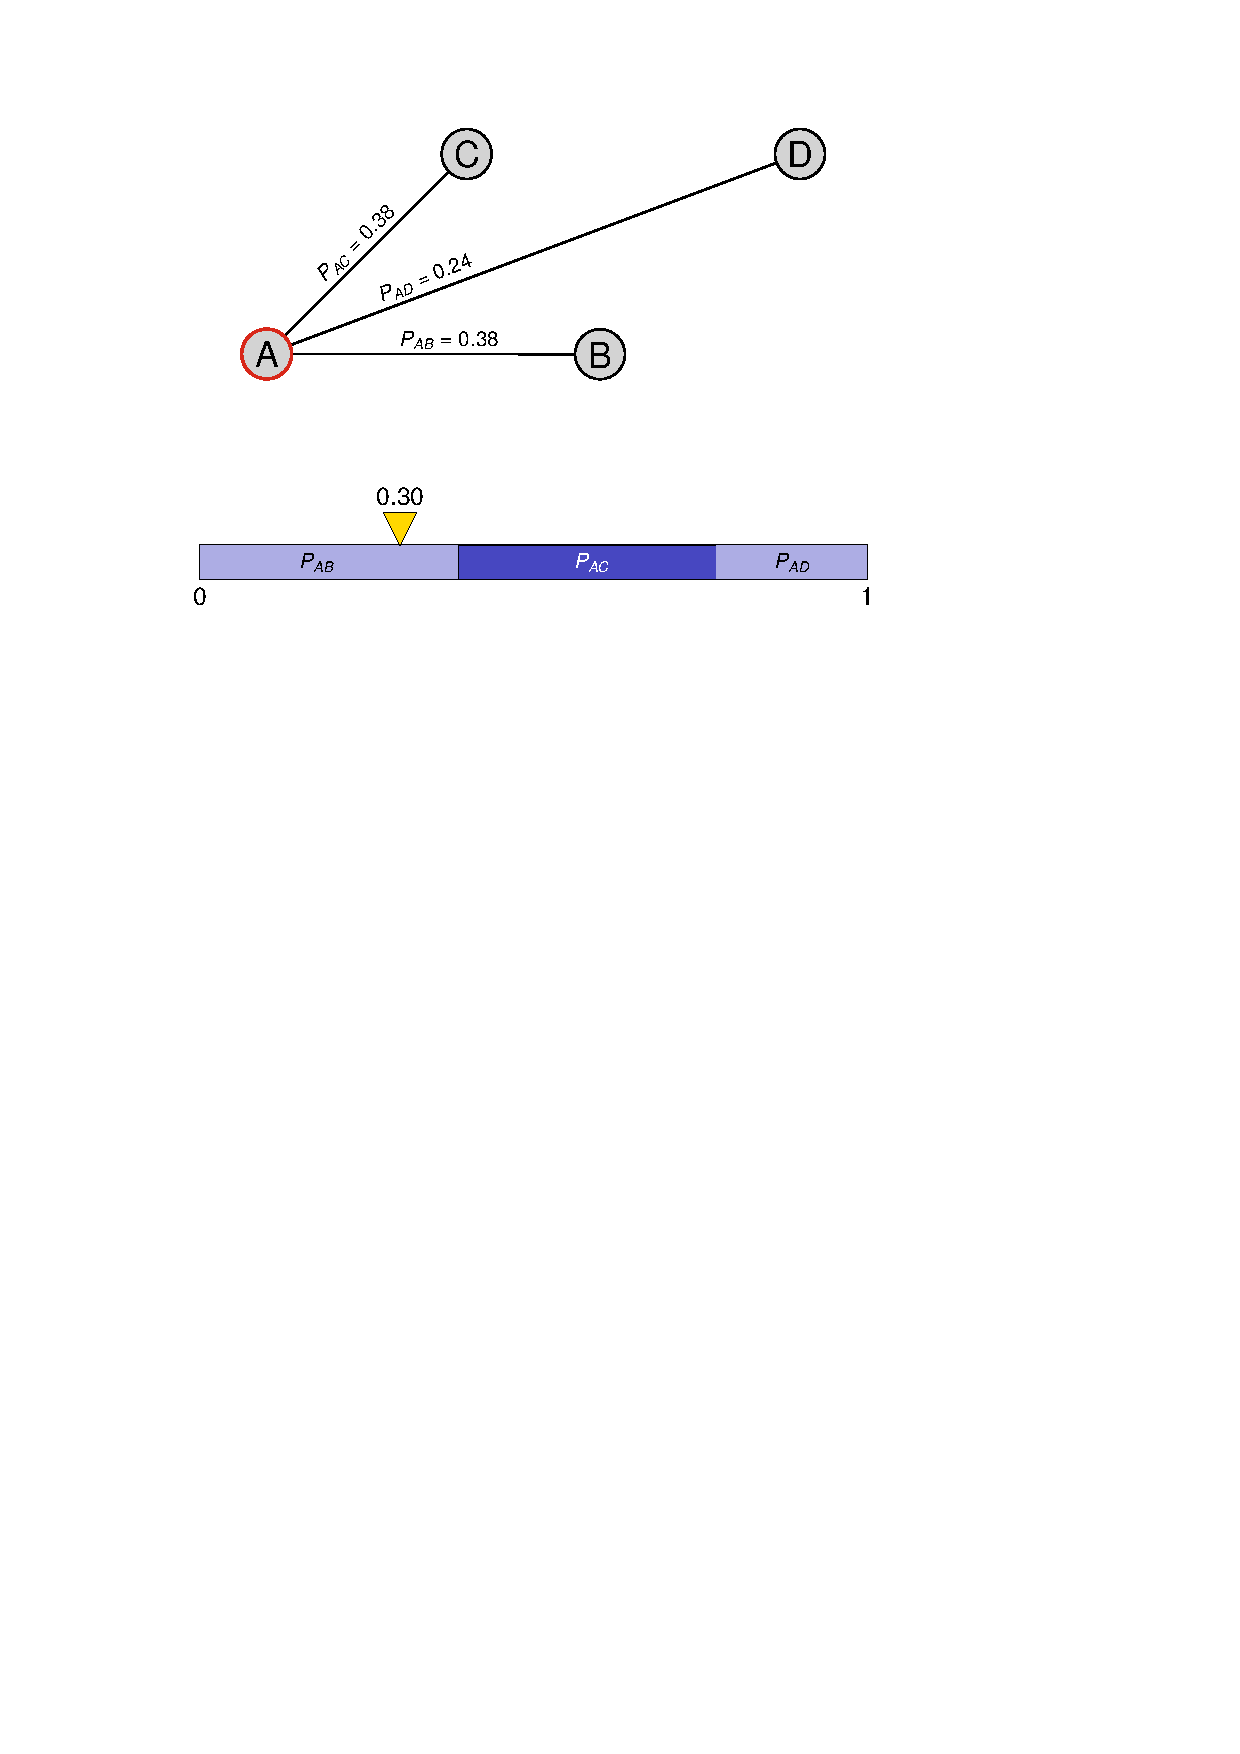
\includegraphics[width=\linewidth, page=1]{aco_probabilities}
		\caption{} \label{subfig:ACO_wahrscheinlichkeiten_a}
	\end{subfigure}
	\begin{subfigure}{0.45\textwidth}
		\includegraphics[width=\linewidth, page=2]{aco_probabilities}
		\caption{} \label{subfig:ACO_wahrscheinlichkeiten_b}
	\end{subfigure}\newline
	\begin{subfigure}{0.55\textwidth}
		\includegraphics[width=\linewidth, page=3, trim=0 100 0 0, clip]{aco_probabilities}
		\caption{} \label{subfig:ACO_wahrscheinlichkeiten_c}
	\end{subfigure}
	\caption{Wegfindung anhand von Wahrscheinlichkeiten und Zufallswerten}
\end{figure}

Im n\"achsten Schritt werden nun die Pheromonwerte aktualisiert, damit sich die Wahrscheinlichkeit, dass folgende Ameisen wieder diesen k\"urzesten Weg gehen, erh\"oht. Dieser Schritt erfolgt in der echten Anwendung erst nachdem alle Ameisen den Iterationsschritt vollendet haben. Um die neuen Pheromonwerte zu berechnen, wird folgende zweiteilige Aktualisierungsregel, bestehend aus Verdunstung und Verst\"arkung, angewandt:
\begin{enumerate}
	\item Die Verdunstung aller Kanten berechnet sich durch
	\[\tau_{ij} = (1 - \rho) \cdot \tau_{ij},\]
	wobei
	\begin{itemize}
		\item $\rho$ die Verdunstungsrate und
		\item $\tau_{ij}$ den Pheromonwert einer Kante darstellt.
	\end{itemize}
	Hierbei werden die Pheromonmengen aller Pfade um einen Faktor, abh\"angig von der verwendeten Verdunstungsrate reduziert. Damit ist es einerseits m\"oglich nicht optimale Entscheidungen zu vergessen. Andererseits k\"onnen sich gute Wege besser absetzen.
	\item Die Verst\"arkung besuchter Kanten l\"asst sich durch
	\[\tau_{ij} = \tau_{ij} + \sum_{k=1}^{m}\frac{Q}{L_k}\]
	berechnen. Hierbei ist
	\begin{itemize}
		\item $Q$ die gesamte Pheromonmenge,
		\item $L_k$ die L\"ange der L\"osung der k-ten Ameisen und
		\item $m$ die Anzahl der Ameisen.
	\end{itemize}
	Mit Hilfe dieser Formel wird jede Kante, die Teil einer L\"osung der k\"unstlichen Ameise ist, durch eine Pheromonmenge relativ zur Qualit\"at der gefundenen Tour verst\"arkt. Angewandt bedeutet das, dass die Kanten einer k\"urzeren Tour mehr Pheromon aufweisen als jene einer l\"angeren Tour.
\end{enumerate}

Mittels dieser Pheromon-Aktualisierung werden kurze gute Wege deutlicher verst\"arkt, was zu erh\"ohten und mit jeder Iteration eindeutigeren Wahrscheinlichkeiten f\"uhrt. Kurze Wege werden mit der Zeit klar bevorzugt [\cref{fig:ACO_aktualisierung}]. \cite[vgl.][]{DorigoStuetzle04}

\begin{figure}[ht]
	\begin{center}
		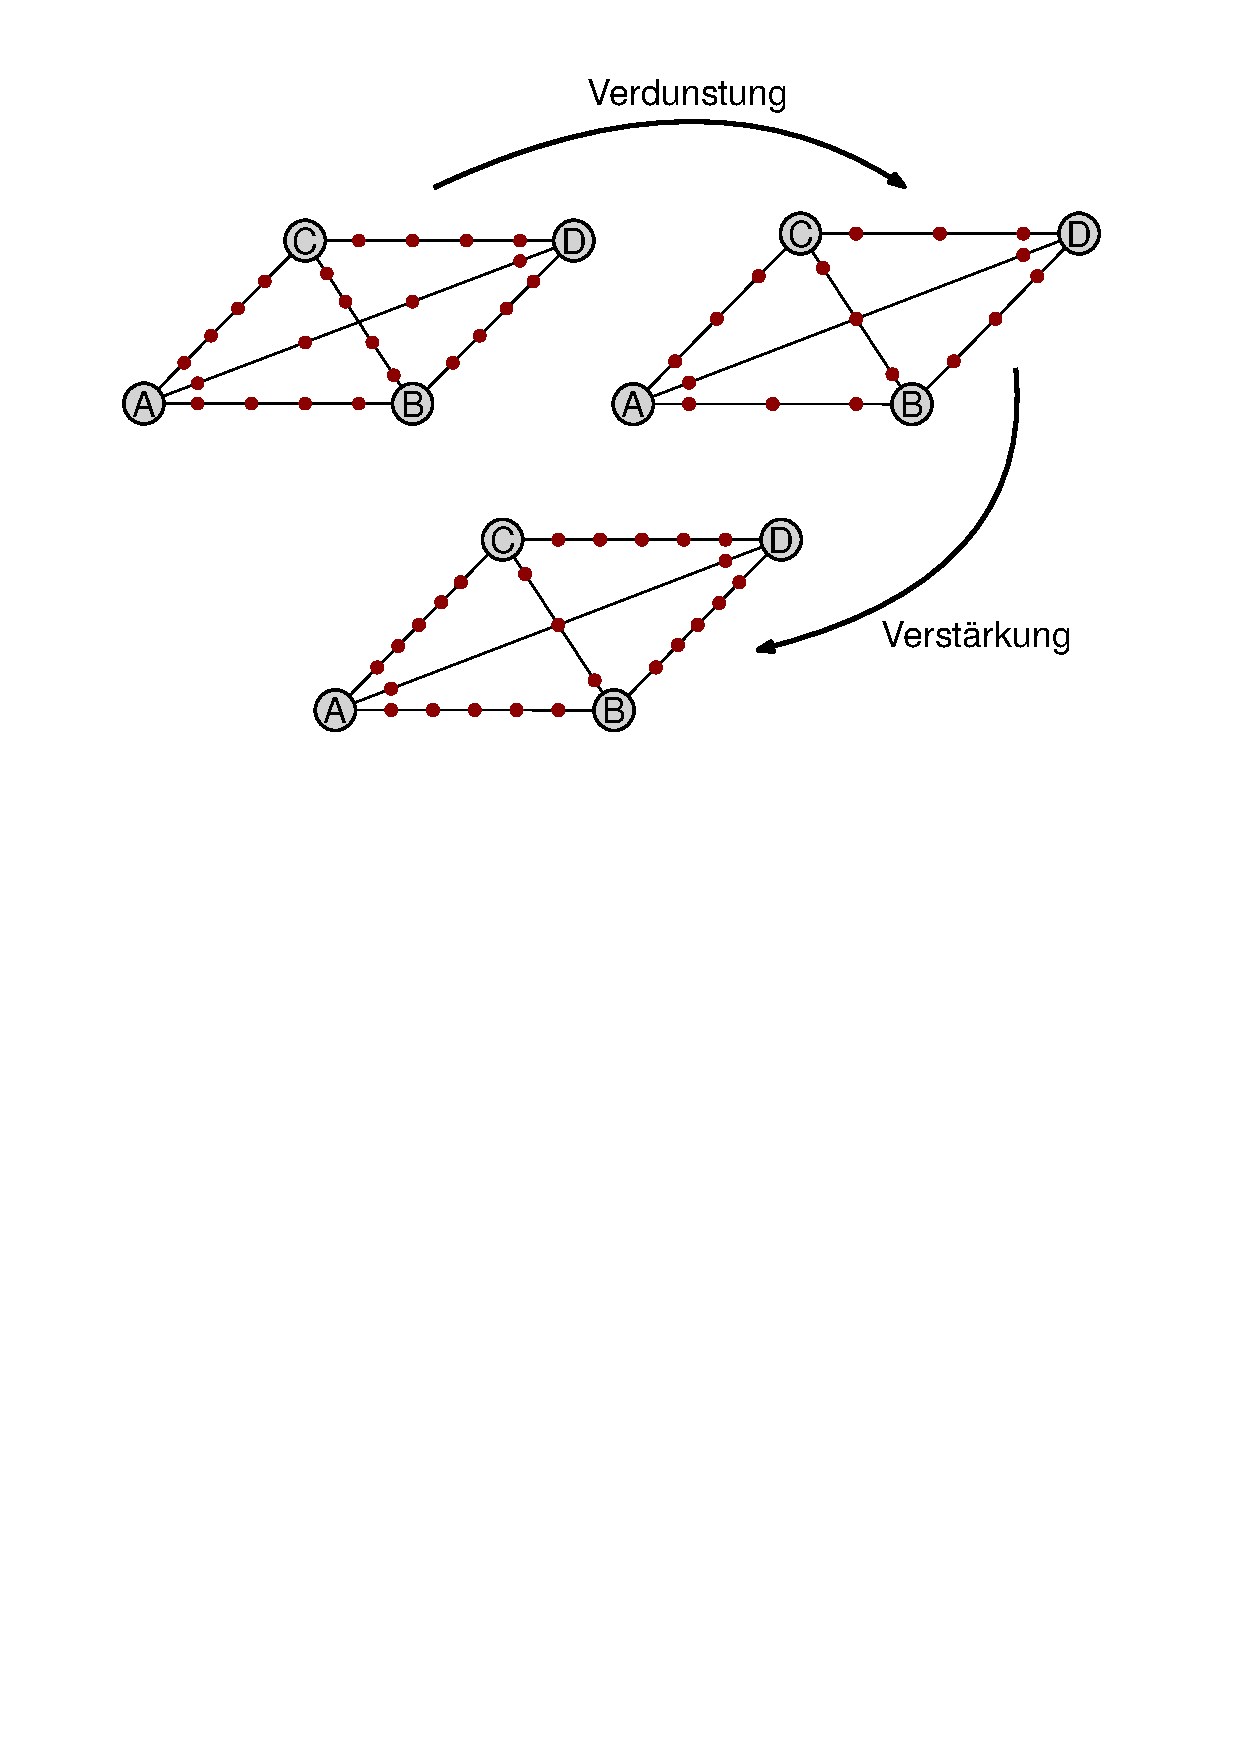
\includegraphics[width=0.8\linewidth]{aco_update}
		\caption{Verdunstung und Verst\"arkung der Kanten} \label{fig:ACO_aktualisierung}
	\end{center}
\end{figure}

Zusammenfassend liegt die St\"arke des ACO in der F\"ahigkeit komplexe kombinatorische Optimierungsprobleme zu l\"osen. Dies findet unter anderem Anwendung im Bereich der Logistik, z.B. bei der Optimierung von Lieferketten und Verkehrsfluss. Aber auch im Netzwerk Routing k\"onnen damit Datenpakete effizient geleitet werden, also z.B. Routen mit geringerer Latenz bevorzugt werden. Ein weiteres Anwendungsgebiet des ACO ist die Planung und Zuteilung knapper Ressourcen z.B. bei der Produktionsplanung. \cite[vgl.][]{DorigoStuetzle04}


\section{Partikelschwarmoptimierung PSO}
\subsection{Biologie}
Biologisch inspiriert ist die Partikelschwarmoptimierung von Fisch- und Vogelschw\"armen. Die Mitglieder eines solchen Schwarmes folgen dabei einfachen Regeln, die in der Folge dann zu einem komplexen globalen Verhalten f\"uhren. Jedes Schwarmmitglied m\"ochte bei seinem Schwarm bleiben, nicht mit den anderen Individuen zusammensto\ss en und sich in die gleiche Richtung bewegen wie die anderen. Fische und auch V\"ogel nutzen dieses Verhalten um die Nahrungssuche zu optimieren aber auch um sich vor Fressfeinden zu sch\"utzen. \cite[vgl.][]{KennedyEberhart01}


\subsection{Algorithmus}
Die Partikelschwarmoptimierung wird verwendet um Extremstellen in multidimensionalen Funktionen zu finden. Diese Funktionen werden auch Suchr\"aume genannt. Der Algorithmus setzt dabei auf die Simulation eines Schwarms von sogenannten Partikeln. Diese Partikel stellen m\"ogliche L\"osungen des Optimierungsproblems dar. Jedes Partikel kennt die Koordinaten seiner aktuellen Position im Suchraum, kann sich mit Hilfe eines Bewegungsvektors bewegen und hat zus\"atzlich ein Ged\"achtnis f\"ur die pers\"onlich beste erreichte Position (kognitive Komponente) und die beste vom Schwarm erreichte Position (soziale Komponente). Der PSO-Algorithmus bestimmt f\"ur  jedes Partikel $i$ des Schwarms die n\"achste Position $P_i$. Dabei wird initial jedem Partikel des Schwarms eine zuf\"allige Position zugewiesen. Des weiteren wird der pers\"onliche Bestwert $P_{pbest(i)^t}$ [\cref{subsec:PSO_kognitiv}] auf die aktuelle Position gesetzt. Der globale Bestwert $P_{gbest^t}$ [\cref{subsec:PSO_sozial}] wird f\"ur den Schwarm berechnet und f\"ur die erste Iteration gespeichert. Bei jedem folgenden Iterationsschritt $t+1$ des Algorithmus wird die Position f\"ur jedes Partikel neu berechnet. Um die n\"achste Position zu bestimmen wird ein Bewegungsvektor verwendet. Der Bewegungsvektor [\cref{fig:PSO_bewegung}] setzt sich aus drei Komponenten zusammen:
\begin{itemize}
	\item Tr\"agheitsmoment $\omega V_i^t$,
	\item Soziale Komponente $c_1r_1\left(P_{pbest(i)^t}-P_i^t\right)$ und
	\item Kognitive Komponente $c_2r_2\left(P_{gbest^t}^t-P_i^t\right)$.
\end{itemize}
Daraus ergibt sich \[V_i^{t+1} = \omega V_i^t + c_1r_1\left(P_{pbest(i)^t}-P_i^t\right) + c_2r_2\left(P_{gbest^t}^t-P_i^t\right)\] als Formel f\"ur den Bewegungsvektor. Die Position der Partikel wird so oft neu berechnet, bis eine Abbruchbedingung erreicht ist. Diese kann zum Beispiel ein f\"ur 50 Iterationen unver\"anderter globaler Bestwert sein. \cite[vgl.][]{KennedyEberhart95, ZhangWangJi15}

\begin{figure}[!ht]
	\centering
	\begin{subfigure}{0.45\textwidth}
		\includegraphics[trim=250 140 200 70, clip, width=\linewidth, page=2]{pso_algorithm_structure}
		\caption{Tr\"agheitskomponente}\label{subfig:PSO_bewegung_traegheit}
	\end{subfigure}
	\begin{subfigure}{0.45\textwidth}
		\includegraphics[trim=250 140 200 70, clip, width=\linewidth, page=3]{pso_algorithm_structure}
		\caption{Kognitive Komponente}\label{subfig:PSO_bewegung_kognitiv}
	\end{subfigure}
	\\
	\begin{subfigure}{0.45\textwidth}
		\includegraphics[trim=250 140 200 70, clip, width=\linewidth, page=4]{pso_algorithm_structure}
		\caption{Soziale Komponente}\label{subfig:PSO_bewegung_sozial}
	\end{subfigure}
	\begin{subfigure}{0.45\textwidth}
		\includegraphics[trim=250 140 200 70, clip, width=\linewidth, page=5]{pso_algorithm_structure}
		\caption{Resultierender Bewegungsvektor}\label{subfig:PSO_bewegung_result}
	\end{subfigure}
	\\
	\begin{tabular}{llrl}
		\tikz\draw[black, fill={rgb,1: red,0.6; green,0.8; blue,0.2}, thick] (0,0) circle (3pt); & Minimum des Suchraumes &
		\tikz\draw[black, fill=white, thick] (0,0) circle (3pt); & globaler Bestwert\\
		\tikz\draw[black, fill=orange, thick] (0,0) circle (3pt); & pers\"onlicher Bestwert &
		\tikz\draw[black, fill=black, thick] (0,0) circle (3pt); & aktuelle Position
	\end{tabular}
	\caption{Berechnung des Bewegungsvektors}\label{fig:PSO_bewegung}
\end{figure}


\subsubsection{Tr\"agheitskomponente}
\label{subsec:PSO_traegheit}
Der Algorithmus verwendet die letzte Bewegung des Partikels f\"ur die n\"achste Bewegung wieder. Die Bewegung wird mit einer Gewichtung $\omega$ versehen und bildet mit dem letzten Bewegungsvektor $V_i^t$ die Tr\"agheitskomponente [\cref{subfig:PSO_bewegung_traegheit}] \cite[vgl.][]{KennedyEberhart01, KennedyEberhart95}, also \[\omega V_i^t.\]


\subsubsection{Kognitive Komponente}
\label{subsec:PSO_kognitiv}
Die kognitive Komponente gibt eine Gewichtung des pers\"onlichen Bestwerts an [\cref{subfig:PSO_bewegung_kognitiv}]. Dabei gewichtet jedes Partikel des Schwarms den eigenen Bestwert individuell. Dies wird mit Hilfe eines Richtungsvektors und zweier Gewichte realisiert. Der Richtungsvektor $P_{pbest(i)^t}-P_i^t$ bildet einen Vektor, welcher vom Partikel in Richtung des pers\"onlichen Bestwertes zeigt. $c_1$ entspricht der kognitiven Gewichtung und ist f\"ur den gesamten Schwarm identisch. $r_1$ ist ein Zufallsfaktor, welcher f\"ur jedes Partikel individuell ist. Die zwei Gewichte werden auf den Richtungsvektor aufmultipliziert und bilden somit einen Skalar. \cite[vgl.][]{KennedyEberhart01, ZhangWangJi15} Daraus folgt \[c_1r_1\left(P_{pbest(i)^t}-P_i^t\right).\]


\subsubsection{Soziale Komponente}
\label{subsec:PSO_sozial}
Die soziale Komponente ist die Gewichtung des globalen Bestwertes [\cref{subfig:PSO_bewegung_sozial}]. Wie die kognitive Komponente aus \cref{subsec:PSO_kognitiv} setzt sich die soziale Komponente aus einem Richtungsvektor und zwei Gewichten zusammen. Der Richtungsvektor entspricht aber $P_{gbest^t}^t-P_i^t$ und ist somit ein Vektor, welcher vom Partikel aus in Richtung des globalen Bestwertes zeigt. Das erste Gewicht $c_2$ ist f\"ur den gesamten Schwarm gleich gew\"ahlt. $r_2$ ist wieder ein Zufallsfaktor.  Die Zusammensetzung dieser Faktoren bildet den skalierten Richtungsvektor \cite[vgl.][]{KennedyEberhart01, ZhangWangJi15} \[c_2r_2\left(P_{gbest^t}^t-P_i^t\right).\]


\subsubsection{Positionsbestimmung}
\label{subsec:PSO_positionsbestimmung}
Die Summe der drei Komponenten der \crefrange{subsec:PSO_traegheit}{subsec:PSO_sozial} bilden den Bewegungsvektor \[V_i^{t+1} = \omega V_i^t + c_1r_1\left(P_{pbest(i)^t}-P_i^t\right) + c_2r_2\left(P_{gbest^t}^t-P_i^t\right)\] welcher die n\"achste Position $P_i^{t+1}$ eines jeden Partikels bestimmt [\cref{subfig:PSO_bewegung_result}]. Die n\"achste Position ist die Summe aus der aktuellen Position und dem Bewegungsvektor \cite[vgl.][]{KennedyEberhart01, ZhangWangJi15} \[P_i^{t+1} = P_i^t + V_i^{t+1}.\]


\subsection{Anwendung des Algorithmus}
\label{subsec:PSO_anwendung}
\begin{figure}[ht]
	\centering
	\begin{subfigure}{0.3\linewidth}
		\includegraphics[trim=220 50 200 50, clip, width=\linewidth, page=1]{pso_swarm_simulation}
		\caption{Initialverteilung $t = 0$}
		\label{subfig:PSO_example_init}
	\end{subfigure}
	\begin{subfigure}{0.3\linewidth}
		\includegraphics[trim=220 50 200 50, clip, width=\linewidth, page=2]{pso_swarm_simulation}
		\caption{$t=10$}
		\label{subfig:PSO_example_2}
	\end{subfigure}
	\begin{subfigure}{0.3\linewidth}
		\includegraphics[trim=220 50 200 50, clip, width=\linewidth, page=3]{pso_swarm_simulation}
		\caption{$t=20$}
	\end{subfigure}\\

	\begin{subfigure}{0.3\linewidth}
		\includegraphics[trim=220 50 200 50, clip, width=\linewidth, page=4]{pso_swarm_simulation}
		\caption{$t=30$}
	\end{subfigure}
	\begin{subfigure}{0.3\linewidth}
		\includegraphics[trim=220 50 200 50, clip, width=\linewidth, page=5]{pso_swarm_simulation}
		\caption{$t=40$}
	\end{subfigure}
	\begin{subfigure}{0.3\linewidth}
		\includegraphics[trim=220 50 200 50, clip, width=\linewidth, page=6]{pso_swarm_simulation}
		\caption{$t=50$}
		\label{subfig:PSO_example_6}
	\end{subfigure}

	\tikz\draw[black, fill=white, thick] (0,0) circle (3pt); globales Minimum
	\caption{Beispiel mit 100 Partikeln}
	\label{fig:PSO_beispiel}
\end{figure}

Diesen Algorithmus kann man nun auf einen ganzen Schwarm anwenden. Dabei wird zuerst der Suchraum definiert. Meist ist dies eine Funktion h\"oherer Dimension. Danach wird die gewollte Menge an Partikeln ($i\in\{0, 1, \dots, N\}\quad N \in\N$) zuf\"allig im Suchraum verteilt. Jedes Partikel wird dabei mit den Werten $c_1, r_1, c_2$ und $r_2$ ausgestattet. Im Anschluss wird der globale Bestwert des Schwarmes bestimmt. Dabei wird die beste Position der Partikel verwendet, welche bei der Suche nach einem Minimum der \glqq kleinste\grqq\, Wert ist. Jedes Partikel setzt zus\"atzlich die aktuelle Position als pers\"onlichen Bestwert fest. Nachdem der Schwarm initialisiert ist, wird die erste Iteration ausgef\"uhrt. Dabei wird iterativ jedes Partikel bewegt. Jedes Partikel berechnet also seinen Bewegungsvektor und bewegt sich mit diesem. Nach der Berechnung der n\"achsten Position wird eventuell der pers\"onliche Bestwert neu gesetzt. Nachdem jedes Partikel die neue Position bestimmt hat, wird der globale Bestwert neu gesetzt. Dabei wird die Position jedes Partikels mit dem globalen Bestwert abgeglichen und eventuell aktualisiert. Diese Schritte werden so lange wiederholt, bis die Abbruchbedingung erreicht ist. \cite[vgl.][]{KennedyEberhart01}

\cref{fig:PSO_beispiel} zeigt einen solchen Vorgang. \cref{subfig:PSO_example_init} stellt dabei den ersten Schritt, die Initialisierung, dar. In den darauffolgenden Schritten \crefrange{subfig:PSO_example_2}{subfig:PSO_example_6} werden Iterationen ausgef\"uhrt. Nach 50 Iterationen befindet sich der Schwarm bereits gut sichtbar beim Minimum des definierten Suchraums. Es befinden sich aber auch drei Partikel im lokalen Minimum neben dem globalen Minimum. Diese Partikel gewichten den pers\"onlichen Bestwert mehr als den globalen Bestwert und sind somit im lokalen Minimum \glqq gefangen\grqq. Die H\"urde zwischen dem lokalen und globalen Minimum ist f\"ur die Partikel nicht \"uberwindbar, wodurch sie in diesem lokalen Minimum bleiben.


\subsection{Code}
Der vollst\"andige Quellcode, mit dem \cref{fig:PSO_bewegung} und \cref{fig:PSO_beispiel} erzeugt wurden, ist auf \url{https://github.com/Kneidl18/PSO} zu finden. Der Code ist in Python geschrieben und wurde eigens von Andreas Auer f\"ur dieses Projekt entwickelt, um die theoretischen Konzepte visuell darzustellen. Dabei werden die Formeln aus \cref{subsec:PSO_positionsbestimmung} als Basis verwendet. Der Code ist unter der MIT-Lizenz und steht zur freien Verf\"ugung.


\subsection{Vor- und Nachteile}
\label{subsec:PSO_vor_nachteile}
Die Partikelschwarmoptimierung stellt ein m\"achtiges Optimierungswerkzeug dar, das vor allem durch seine Robustheit bei komplexen, mehrdimensionalen Suchr\"aumen gl\"anzt. Der Algorithmus ist trotzdem simpel und einfach zu implementieren, da er wenige Parameter besitzt. Trotz der wenigen Parameter reagiert der Algorithmus sehr empfindlich und kann bei falscher Einstellung zu schlechten Leistungen f\"uhren. Ebenso besteht das Problem, die gesuchte globale Extremstelle nicht zu finden und stattdessen eine lokale Extremstelle zu pr\"aferieren, wie es in \cref{subsec:PSO_anwendung} beschrieben ist.


\section{Fazit}
Das Konzept der Schwarmintelligenz zeigt wie mit einfachen, lokal befolgten Regeln komplexe Probleme effizient gel\"ost werden k\"onnen. Dies ist eine der zentralen Lektionen aus der Natur, die sich in der Informatik nutzen lassen. Die vorgestellten Algorithmen demonstrieren, wie eine Umsetzung in der Praxis aussehen kann. Der Ant Colony Optimization (ACO) Algorithmus eignet sich dabei besonders gut f\"ur diskrete Optimierungsprobleme, wie beispielsweise dem Suchen der k\"urzesten Route bei der Routenplanung. Der Particle Swarm Optimization (PSO) Algorithmus hingegen eignet sich f\"ur kontinuierliche Optimierungsprobleme wie beispielsweise die Anpassung einer Route an die aktuellen Verkehrsverh\"altnisse.

\listoffigures

\bibliography{Schwarmintelligenz}
\bibliographystyle{alpha}

\end{document}